\documentclass[12pt]{article}
\usepackage{graphicx}

\begin{document}
    {\Huge \textbf{Young Modulus Practical} \par}
    
    \section*{Formulas}
    \begin{enumerate}
        \item Young Modulus $E = \frac{\sigma}{\epsilon} \; \left(\frac{stress}{strain}\right)$
        \item Stress $\sigma = \frac{F}{A} \; \left(\frac{force}{area}\right)$
        \item Strain $\epsilon = \frac{x}{L} \; \left(\frac{change \: in \: length}{length}\right)$
        \item Weight $W = mg \; \left(mass \times gravity\right)$
    \end{enumerate}

    \section*{Method}
    \begin{enumerate}
        \item Attach pulley at edge of desk
        \item Trap one end of copper wire between 2 wooden blocks 3m away from pulley
        \item Pass wire through pulley and attach mass hanger
        \item Measure diameter $d$ of wire
        \item Place meter ruler under wire and add sticky label to a point. This is the point
        you will be measuring the extension of.
        \item Measure length of wire $L$ from wooden blocks to sticky label
        \item Add different masses and measure the extension of the wire
    \end{enumerate}

    \newpage

    \begin{figure}[h]
        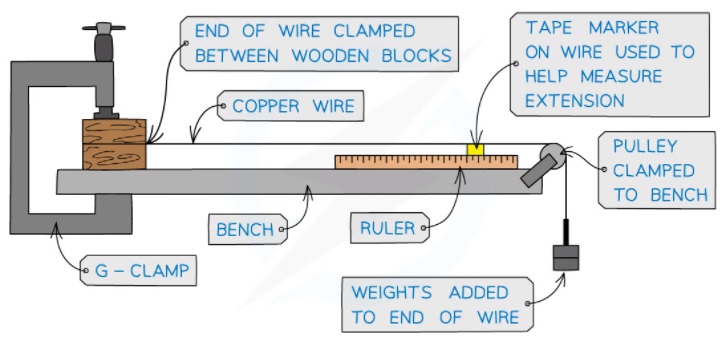
\includegraphics[width = \linewidth]{YoungModul.jpg}
    \end{figure}

    \section*{Making sure everything is accurate}
    \begin{enumerate}
        \item In step 4, measure the diameter in 5 places and take the average
        \item Longer wire will produce a longer extension so less uncertainty in measurement
        \item In step 6 and 7, when measuring the lengths make sure to look vertically down
        over the sticky label and use a set square to make the measurement. This helps avoid
        parallax error
        \item Don't add masses that are too high otherwise there will be creep occuring. Creep is
        basically permanent deformation of the material.
        \item For more data points before the elastic limit of the wire use weights increasing in
        smaller increments. (25g, 50g, 75g instead of 100g, 200g, 300g)
    \end{enumerate}

    \section*{Why a wire?}
    Let's sub in stress and strain formulas into formula for Young Modulus. We get that:
    \[ E = \frac{\frac{F}{A}}{\frac{x}{L}} \]
    \[ \frac{xE}{L} = \frac{F}{A} \]
    \[ x = \frac{FL}{EA} \]
    The Young Modulus $E$ is just a number for copper. We cannot make the force $F$ 
    (weight of mass) too big as that would require huge weights. We can change $A$ (cross 
    sectional area) and $L$ length of material. We want to maximise $x$ (the extension) because
    this is what we measure and this is maximised by minimising $A$ and maximising $L$ which is
    a wire.

    %speak about significant figures

    \section*{How to work out Young Modulus}
    Making $F$ the subject of the formula from the equation in the Why a wire? section we get
    \[ F = x \left(\frac{EA}{L}\right) \]
    And so if we plot force $F$ against extension $x$ our gradient will be $EA/L$. We have measurements
    for $A$ and $L$ so we can work out $E$.

    \section*{Equipment}
    \begin{itemize}
        \item Copper wire
        \item 2 wooden blocks and a clamp
        \item Bench pulley
        \item Mass hanger and slotted masses up to 600g
        \item Metre ruler
        \item Micrometer screw gauge
        \item Sticky label
        \item Set square
    \end{itemize}

    \section*{Safety}
    \begin{enumerate}
        \item Wire is under tension so must wear goggle in case the wire snaps
        \item Take care while adding and removing masses (they may drop)
    \end{enumerate}

    \section*{PS}
    Make sure to convert all the units to meters from millimeters and kilograms
    from grams.
\end{document}